
	\newpage
% =========================================================	
	\section{Kondition} \label{chap:kondition}
% =========================================================
	
	\defi{
		\n
		Die Kondition beschreibt das Fehlerverhältnis zwischen Eingabe und Ausgabe. Man spricht von "guter" oder "schlechter" Kondition, es ist also ein qualitativer Begriff.
		\n 
		Die berechenbare Zahl, die Konditionszahl, entspricht dem ungünstigsten Faktor der Störung. Eine hohe Kondition bedeutet, dass ein Fehler in der Eingabe zu einem noch viel höherem Fehler in der Ausgabe führt.
		Die relative Konditionszahl $\cond(f, x)$ wird folgendermaßen in Abhängigkeit von einer Funktion $f(x)$ berechnet:
		\begin{align} 
	 		\cond(f,x) = \abs{\frac{x \cdot f'(x)}{f(x)}}
	 	\end{align}
		Man unterscheidet generell folgende Fälle:
		\begin{itemize}
			\item $\cond(f, x) \le 1$\\
				Da die Kondition den Fehlerfaktor beschreibt, bedeutet eine Eins, dass es maximal zu keiner Zunahme des relativen Fehlers kommt. Es ist "gut konditioniert".
			\item $\cond(f, x) \gg 1$\\
				Der Fehlerfaktor ist deutlich größer eins und nimmt somit zu. Die Funktion ist "schlecht konditioniert".
				%In diesem speziellen Fall ist die Funktion sehr gut konditioniert, da der Fehler sogar abnimmt.
		\end{itemize}
		%
		\begin{figure}[H]
			\centering
			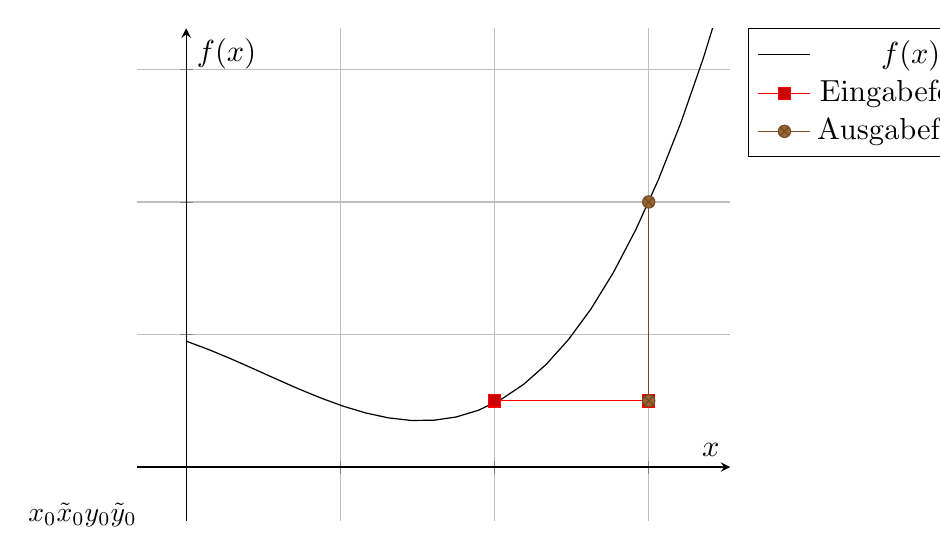
\begin{tikzpicture}[scale=1.1]
				\begin{axis}[
					axis lines=middle,
					xlabel=$x$,
					ylabel=$f(x)$,
					enlargelimits,
					legend pos=outer north east,
					%cycle list name=black white,
					grid=major,
					ymax=6,
					ymin=-0.2,
					xticklabels={,,},
				 	yticklabels={,,},
					]
					\addplot[domain=0:3.5] {1.9 - 0.8*x - 0.5*x^2 + (1/3)*x^3} node[left]{};
					\addplot coordinates {
						( 2, 1 )
						( 3, 1 )
					};
					\addplot coordinates {
						( 3.0, 1 )
						( 3.0, 4 )
					};
					\tikzPointDL{$x_0$}{2,0}
					\tikzPointDL{$\tilde{x}_0$}{3,0}
					\tikzPointUL{$y_0$}{0,1}
					\tikzPointUL{$\tilde{y}_0$}{0,4}
					\legend{$f(x)$, Eingabefehler, Ausgabefehler}
				\end{axis}
			\end{tikzpicture}
			\caption{Plot einer Funktion $f(x)$ und ein Beispiel, wie die Kondition funktioniert. Die exakte Eingabe sei $x_0 = 2$ und wurde durch vorherige Operationen verfälscht ($\tilde{x}_0$). Die Differenz $\abs{\tilde{x}_0 - x_0}$ nennt man den \fat{Eingabefehler}. Dieser führt zu einer Veränderung der Ausgabe, also des $y$-Wertes. Der sogenannte \fat{Ausgabefehler} beschreibt dann die Differenz zwischen der verfälschten Ausgabe $\tilde{y}_0$ und der exakten $y_0$.}
		\end{figure}
	}

	\sbreak
	\bsp{
		\begin{itemize}
			\item $f(x) = x$
				\begin{align*} 
					\cond(f, x) = \abs{\frac{x \cdot 1}{x}} = 1  &&\Longrightarrow \text{gut konditioniert}
				\end{align*}
				Logisch, weil wir die Eingabe ja gerade wieder ausgeben. Wie soll sich da der Fehler der Eingabe überhaupt verändern?
				\sbreak
			\item $g(x) = x^2$
				\begin{align*} 
	 				\cond(g, x) = \abs{\frac{x \cdot 2x}{x^2}} = \frac{2x^2}{x^2} = 2 && \Longrightarrow \text{immer noch gut konditioniert}
	 			\end{align*} 
	 			\sbreak
			\item $h(x) = e^x$
				\begin{align*} 
	 				\cond(h, x) = \abs{\frac{x \cdot e^x}{e^x}} = \abs{x}
	 			\end{align*}
				Fallunterscheidung:
				\begin{align*}
					&\abs{x} \le 1 && \Longrightarrow \text{gut konditioniert} \\
					&\abs{x} \gg 1 && \Longrightarrow \text{schlecht konditioniert}
				\end{align*}
				\sbreak
			\item $i(x) = 1$
				\begin{align*} 
	 				\cond(i, x) = \abs{\frac{x \cdot 0}{1}} = 0 && \Longrightarrow \text{Fehler sind irrelevant}
	 			\end{align*}
				Es ist "perfekt konditioniert". Logisch, da die Ausgabe nicht abhängig von der Eingabe ist. Wie soll die Ausgabe also von einem Eingabefehler überhaupt beeinflusst werden?
		\end{itemize}
	}
